% =================================================================================================
% File:			dp_comportamentali.tex
% Description:	Defiinisce la sezione relativa a ...
% Created:		2015-03-26
% Author:		Tesser Paolo
% Email:		tesser.paolo@mashup-unipd.it
% =================================================================================================
% Modification History:
% Version		Modifier Date		Change											Author
% 0.0.1 		2015-03-26 			sistemato header								Tesser Paolo
% =================================================================================================
% 0.0.2			2015-04-14			descritit DP Page Controller, Template View		Tesser Paolo
% =================================================================================================
% 0.0.3			2015-04-14			descritto DP Template Method					Tesser Paolo
% =================================================================================================
%

% CONTENUTO DEL CAPITOLO

\subsection{Design pattern comportamentali} % (fold)
\label{sub:design_pattern_comportamentali}

	\subsubsection{Page Controller} % (fold)
	\label{ssub:page_controller}
	\begin{itemize}
		\item \textbf{Scope dell'utilizzo}: questo pattern serve per definire un oggetto che detiene le richieste per una specifica pagina o per un'azione su un sito web. In AngularJS però questo componente è maggiormente limitato in quanto al controller sono affidate meno responsabilità quali l'interazione con l'utente e l'aggiornamento del model, mentre la parte delle richieste è lasciato a servizi come \$route o \$state;
		\item \textbf{Contesto dell'utilizzo}:
			\begin{itemize}
				\item \textbf{Client}: viene utilizzato tra tutti i template HTML e i controller associati ad essi. L'associazione viene definita principalmente nei file che si occupano del routing. \newline
				Non ne viene fornita alcuna illustrazione in quanto lo schema è molto simile a quello presentato per il pattern Template View, reperibile alla sezione \ref{ssub:template_view}, solo che il focus nel pattern non è sul template HTML, bensì sul controller che lo gestisce.
			\end{itemize}
	\end{itemize}
	% subsubsection page_controller (end)


	\subsubsection{Template View} % (fold)
	\label{ssub:template_view}
		\begin{itemize}
			\item \textbf{Scope dell'utilizzo}: questo pattern serve per interpretare alcune informazioni incorporate nei template HTML. Nei sistemi di template generalmente vengono utilizzati dei segnaposto (markers) di qualche formato che verranno interpretati e sostituiti con il codice HTML adeguato. In AngularJS invece non c'è un formato intermediario perché vengono usate direttamente delle direttive HTML che quando saranno trovate dal compilatore di Angular, verrà invocata la logica ad esse associata;
			\item \textbf{Contesto dell'utilizzo}:
				\begin{itemize}
					\item \textbf{Client}: viene utilizzato in tutti i template HTML presentati nel package \texttt{client::view} presente alla sezione \ref{ssub:bdsm_app_client_view}. \newline
					Ne viene qui di seguito illustrata una implementazione relativa al template HTML \texttt{Settings}. \newline
					\begin{figure}[!htbp]
						\centering
						\centerline{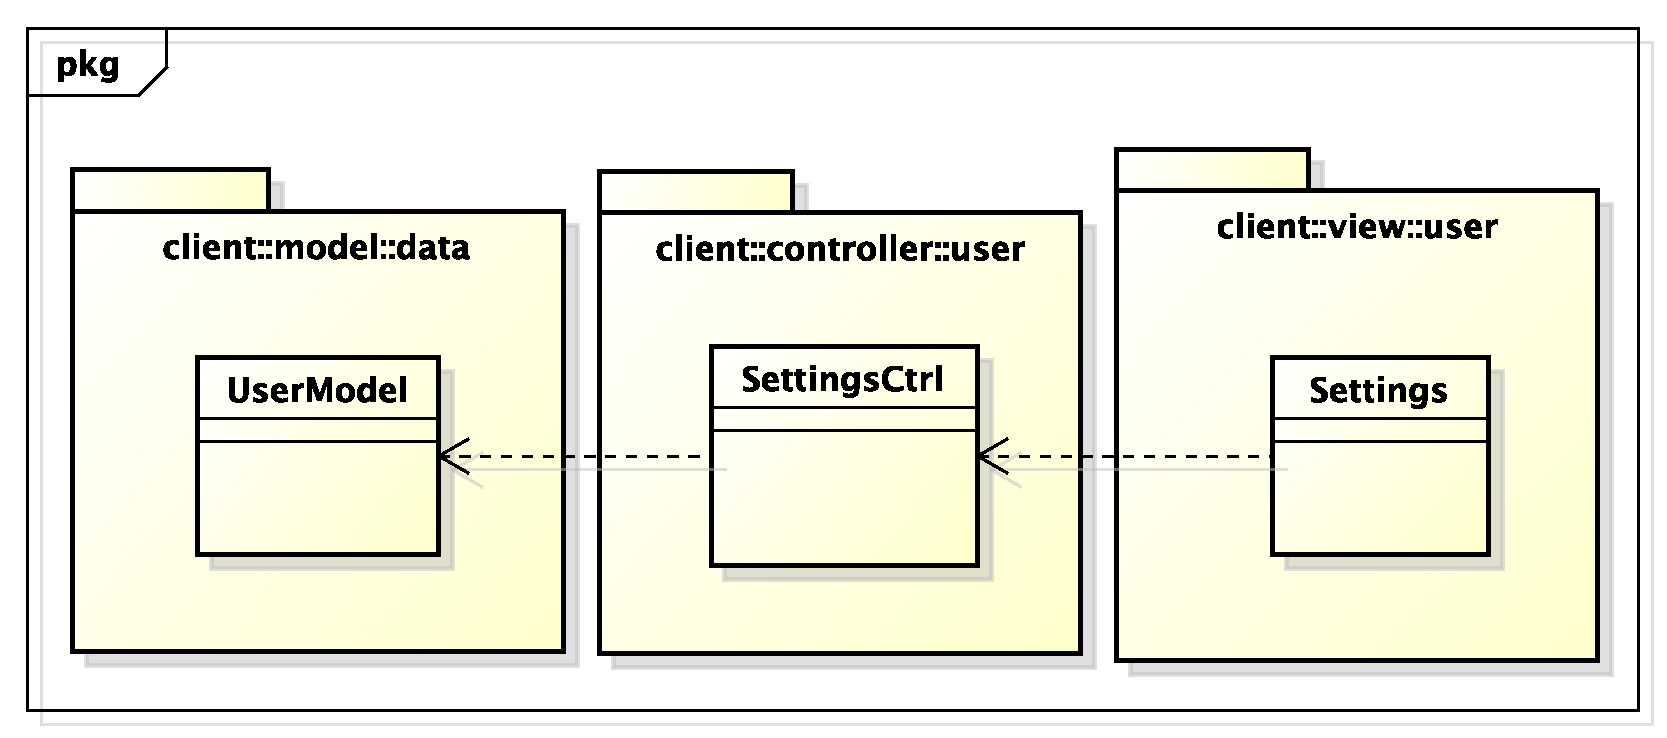
\includegraphics[scale=0.50]{./images/design_pattern_client/client_template_view.pdf}}
						\caption{Contestualizzazione Template View - Client}
					\end{figure}
				\end{itemize}
		\end{itemize}
	% subsubsection template_view (end)


	\subsubsection{Command} % (fold)
	\label{ssub:command}
		\begin{itemize}
			\item \textbf{Scope dell'utilizzo}: questo pattern è utilizzato per incapsulare la logica di una richiesta in un comando totalmente indipendente dall'oggetto che lo invoca. In questo modo si crea una separazione tra logica di esecuzione della richiesta e quella di invocazione, oltre a facilitare l'estensibilità dei comandi associati;
			\item \textbf{Contesto dell'utilizzo}:
				\begin{itemize}
					\item \textbf{Server}: viene utilizzato nel package \texttt{server::processor} in associazione al pattern Front Controller, il cui il dispatcher si occupa di indirizzare la richiesta ricevuta al relativo comando. \newline
					\begin{figure}[!htbp]
						\centering
						\centerline{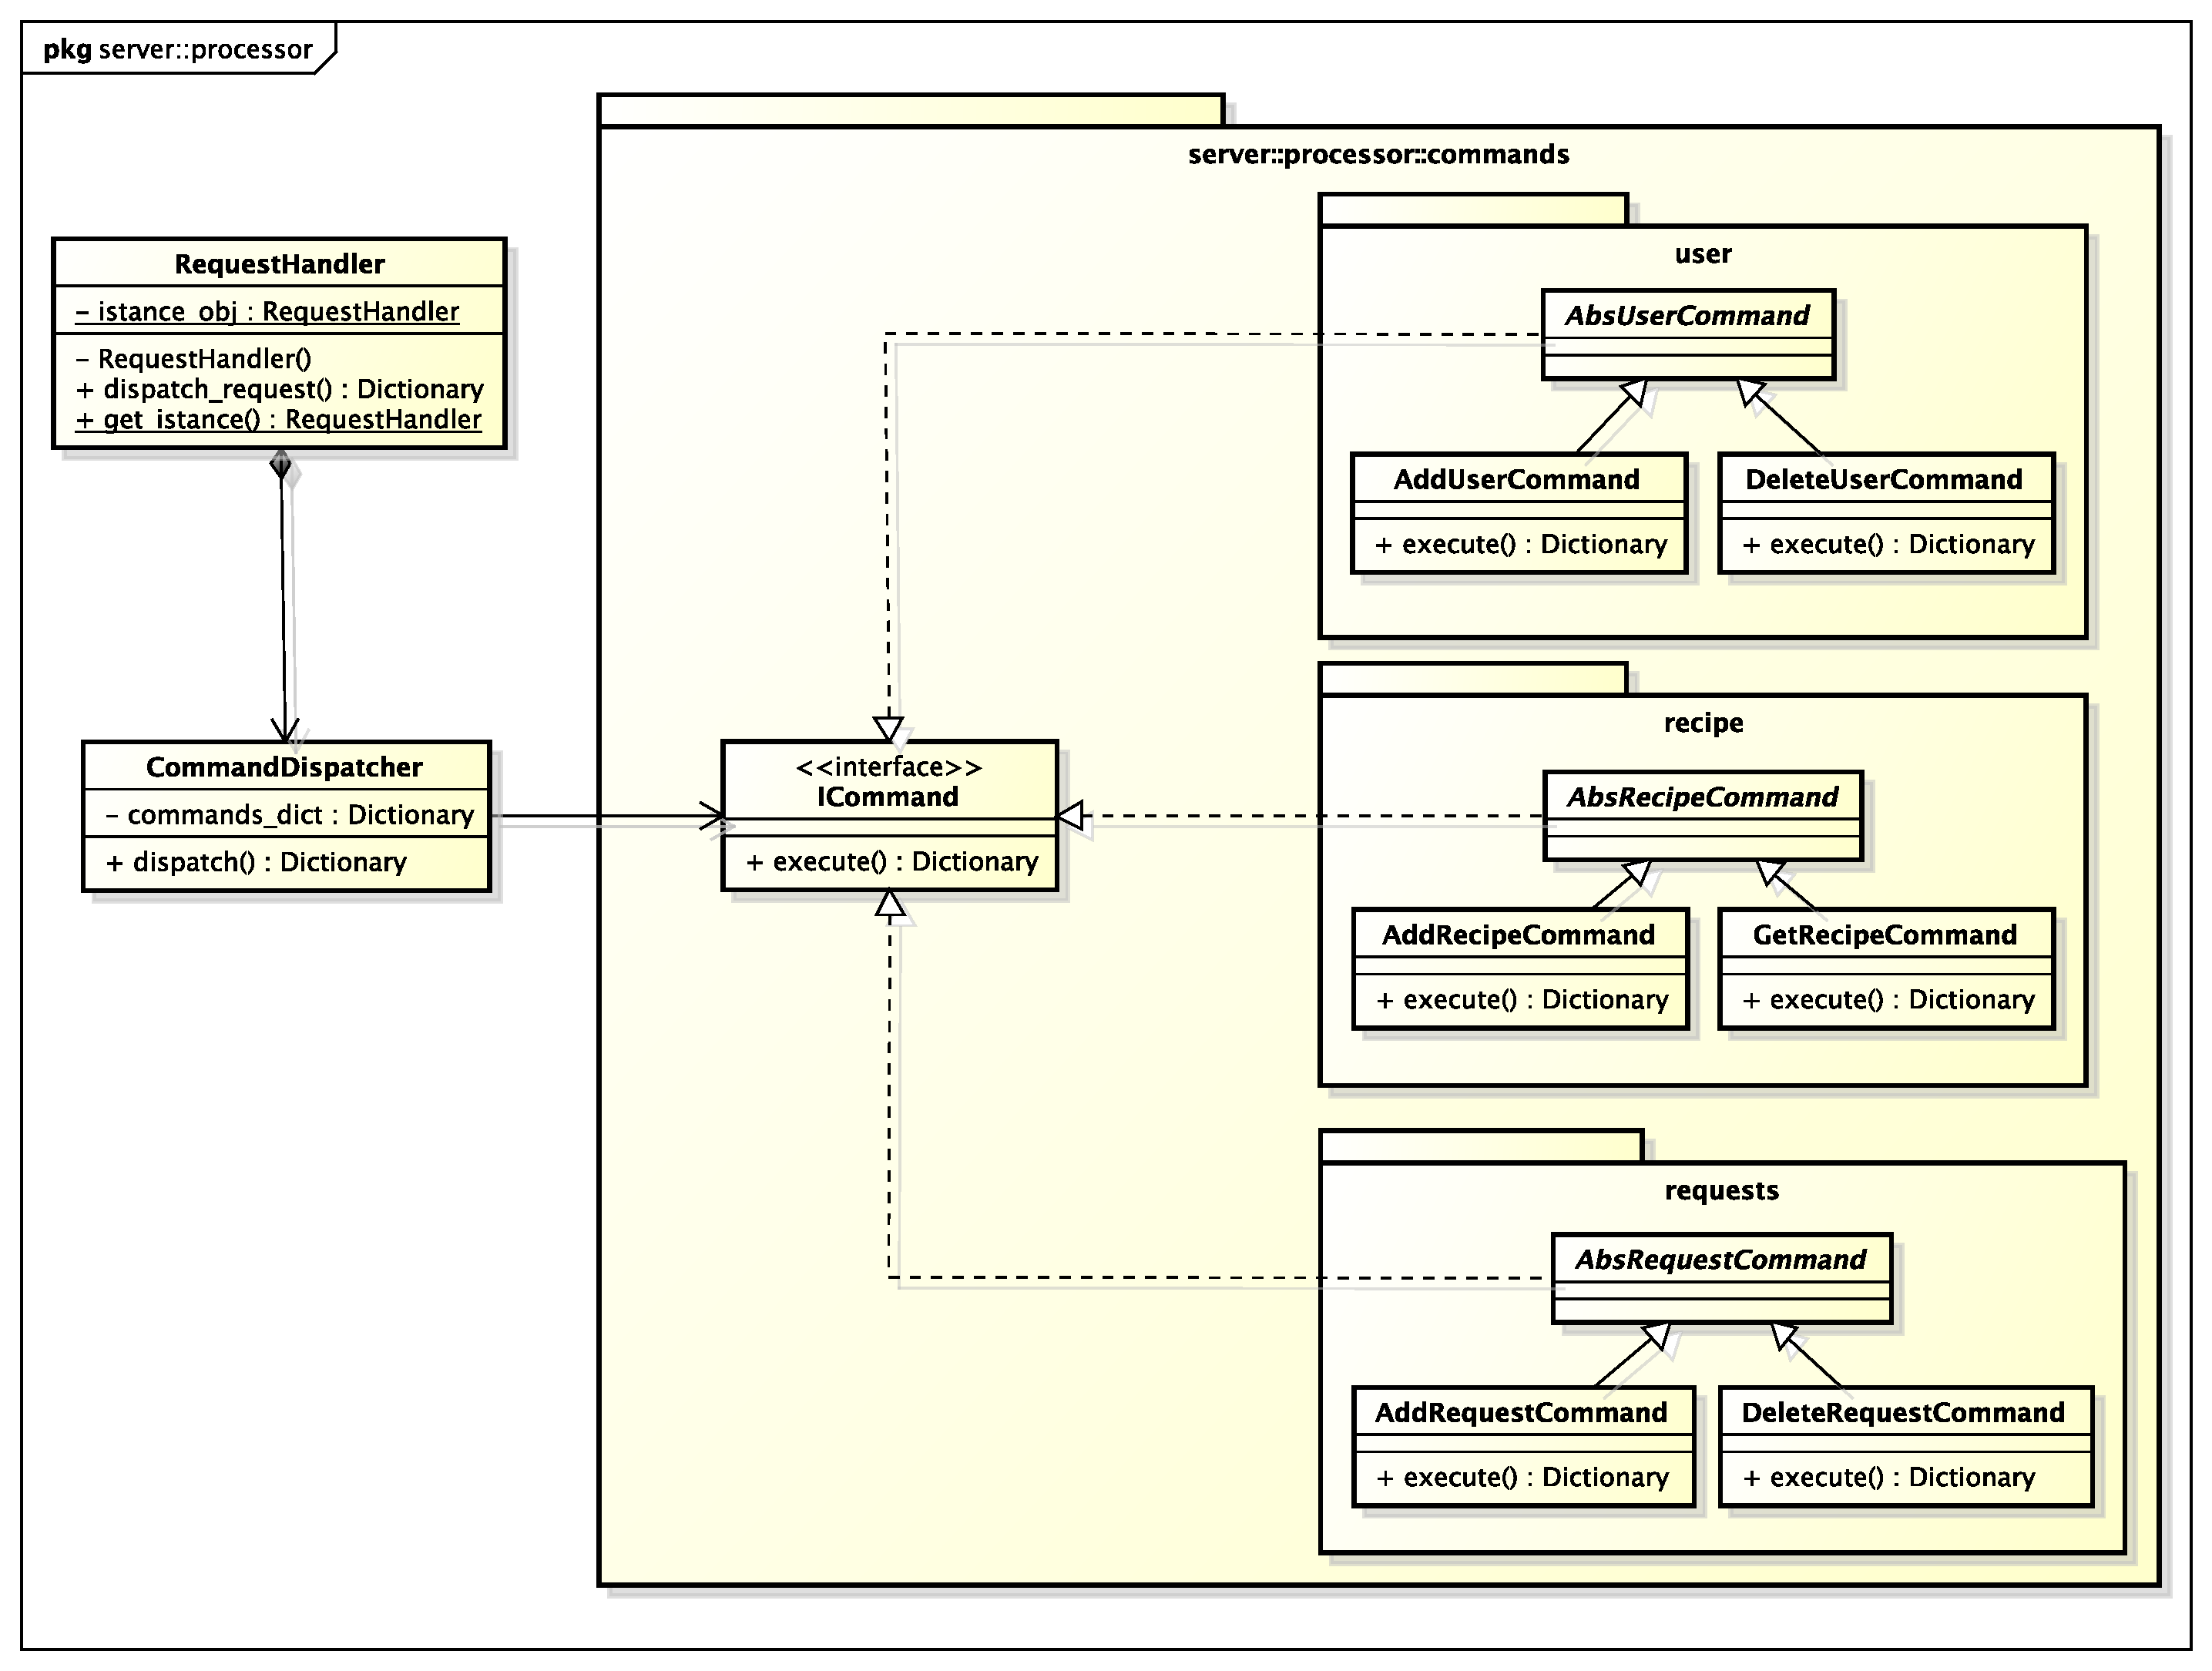
\includegraphics[scale=0.35]{./images/design_pattern_server/dp_command.pdf}}
						\caption{Contestualizzazione Command - Server}
					\end{figure}
				\end{itemize}
		\end{itemize}
	% subsubsection command (end)


	\subsubsection{Template Method} % (fold)
	\label{ssub:template_method}
		\begin{itemize}
			\item \textbf{Scope dell'utilizzo}: questo pattern serve per definire lo scheletro di un algoritmo, lasciando l'implementazione di alcuni passi alle sottoclassi;
			\item \textbf{Contesto dell'utilizzo}:
				\begin{itemize}
					\item \textbf{Client}: viene utilizzato nel package \ref{ssub:bdsm_app_client_model_services}, per permettere di generare tipi di grafici diversi che però hanno in comune la prima parte dell'algoritmo che li genera. In particolare la parte comune si occupa del recupero dei dati a prescindere da quali grafico li userà.
					\begin{figure}[!htbp]
						\centering
						\centerline{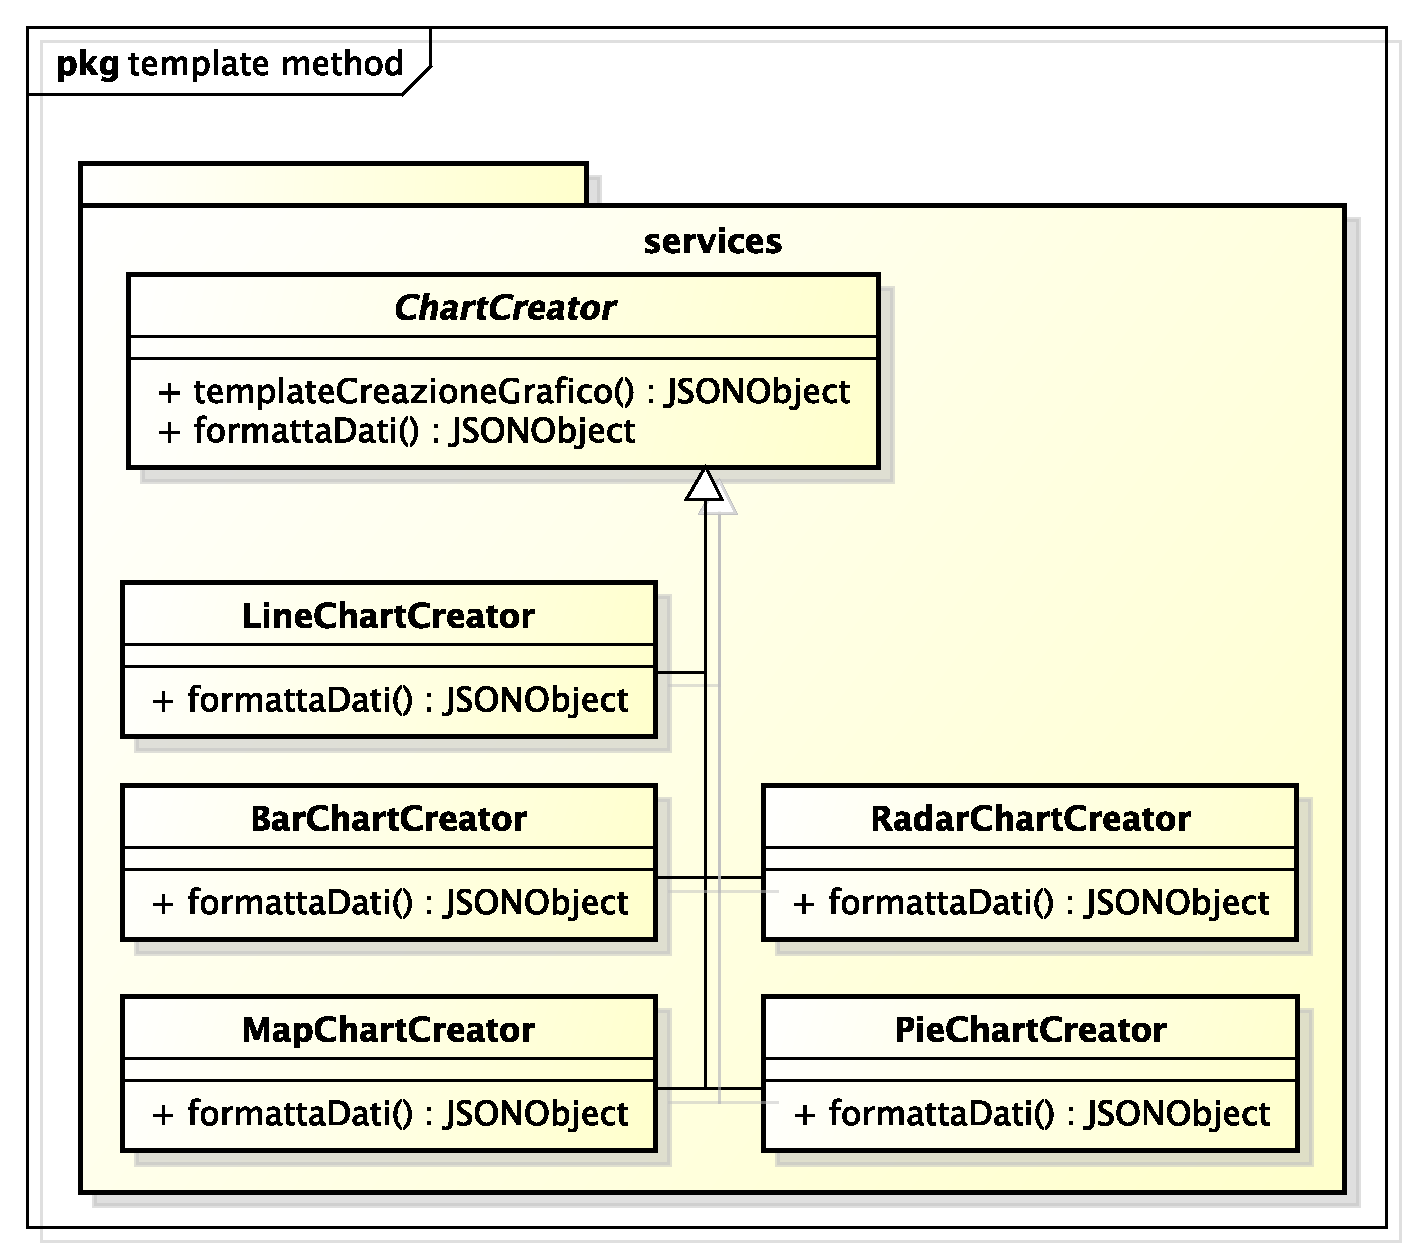
\includegraphics[scale=0.40]{./images/design_pattern_client/client_template_method.pdf}}
						\caption{Contestualizzazione Template Method - Client}
					\end{figure}

					\item \textbf{Server}: viene utilizzato nel package \texttt{server::miner}, implementato dalla gerarchia di classi con \texttt{AbsCounter} come classe padre. L'algoritmo serve ad effettuare il counting di differenti entità ottenute tramite le API dei vari social network al fine di ottenere i dati grezzi richiesti. L'algoritmo contiene uno scheletro comune esposto dalla classe padre e viene implementato a seconda del social e del dato di cui si vuole effettuare il conteggio. \newline
					\begin{figure}[!htbp]
						\centering
						\centerline{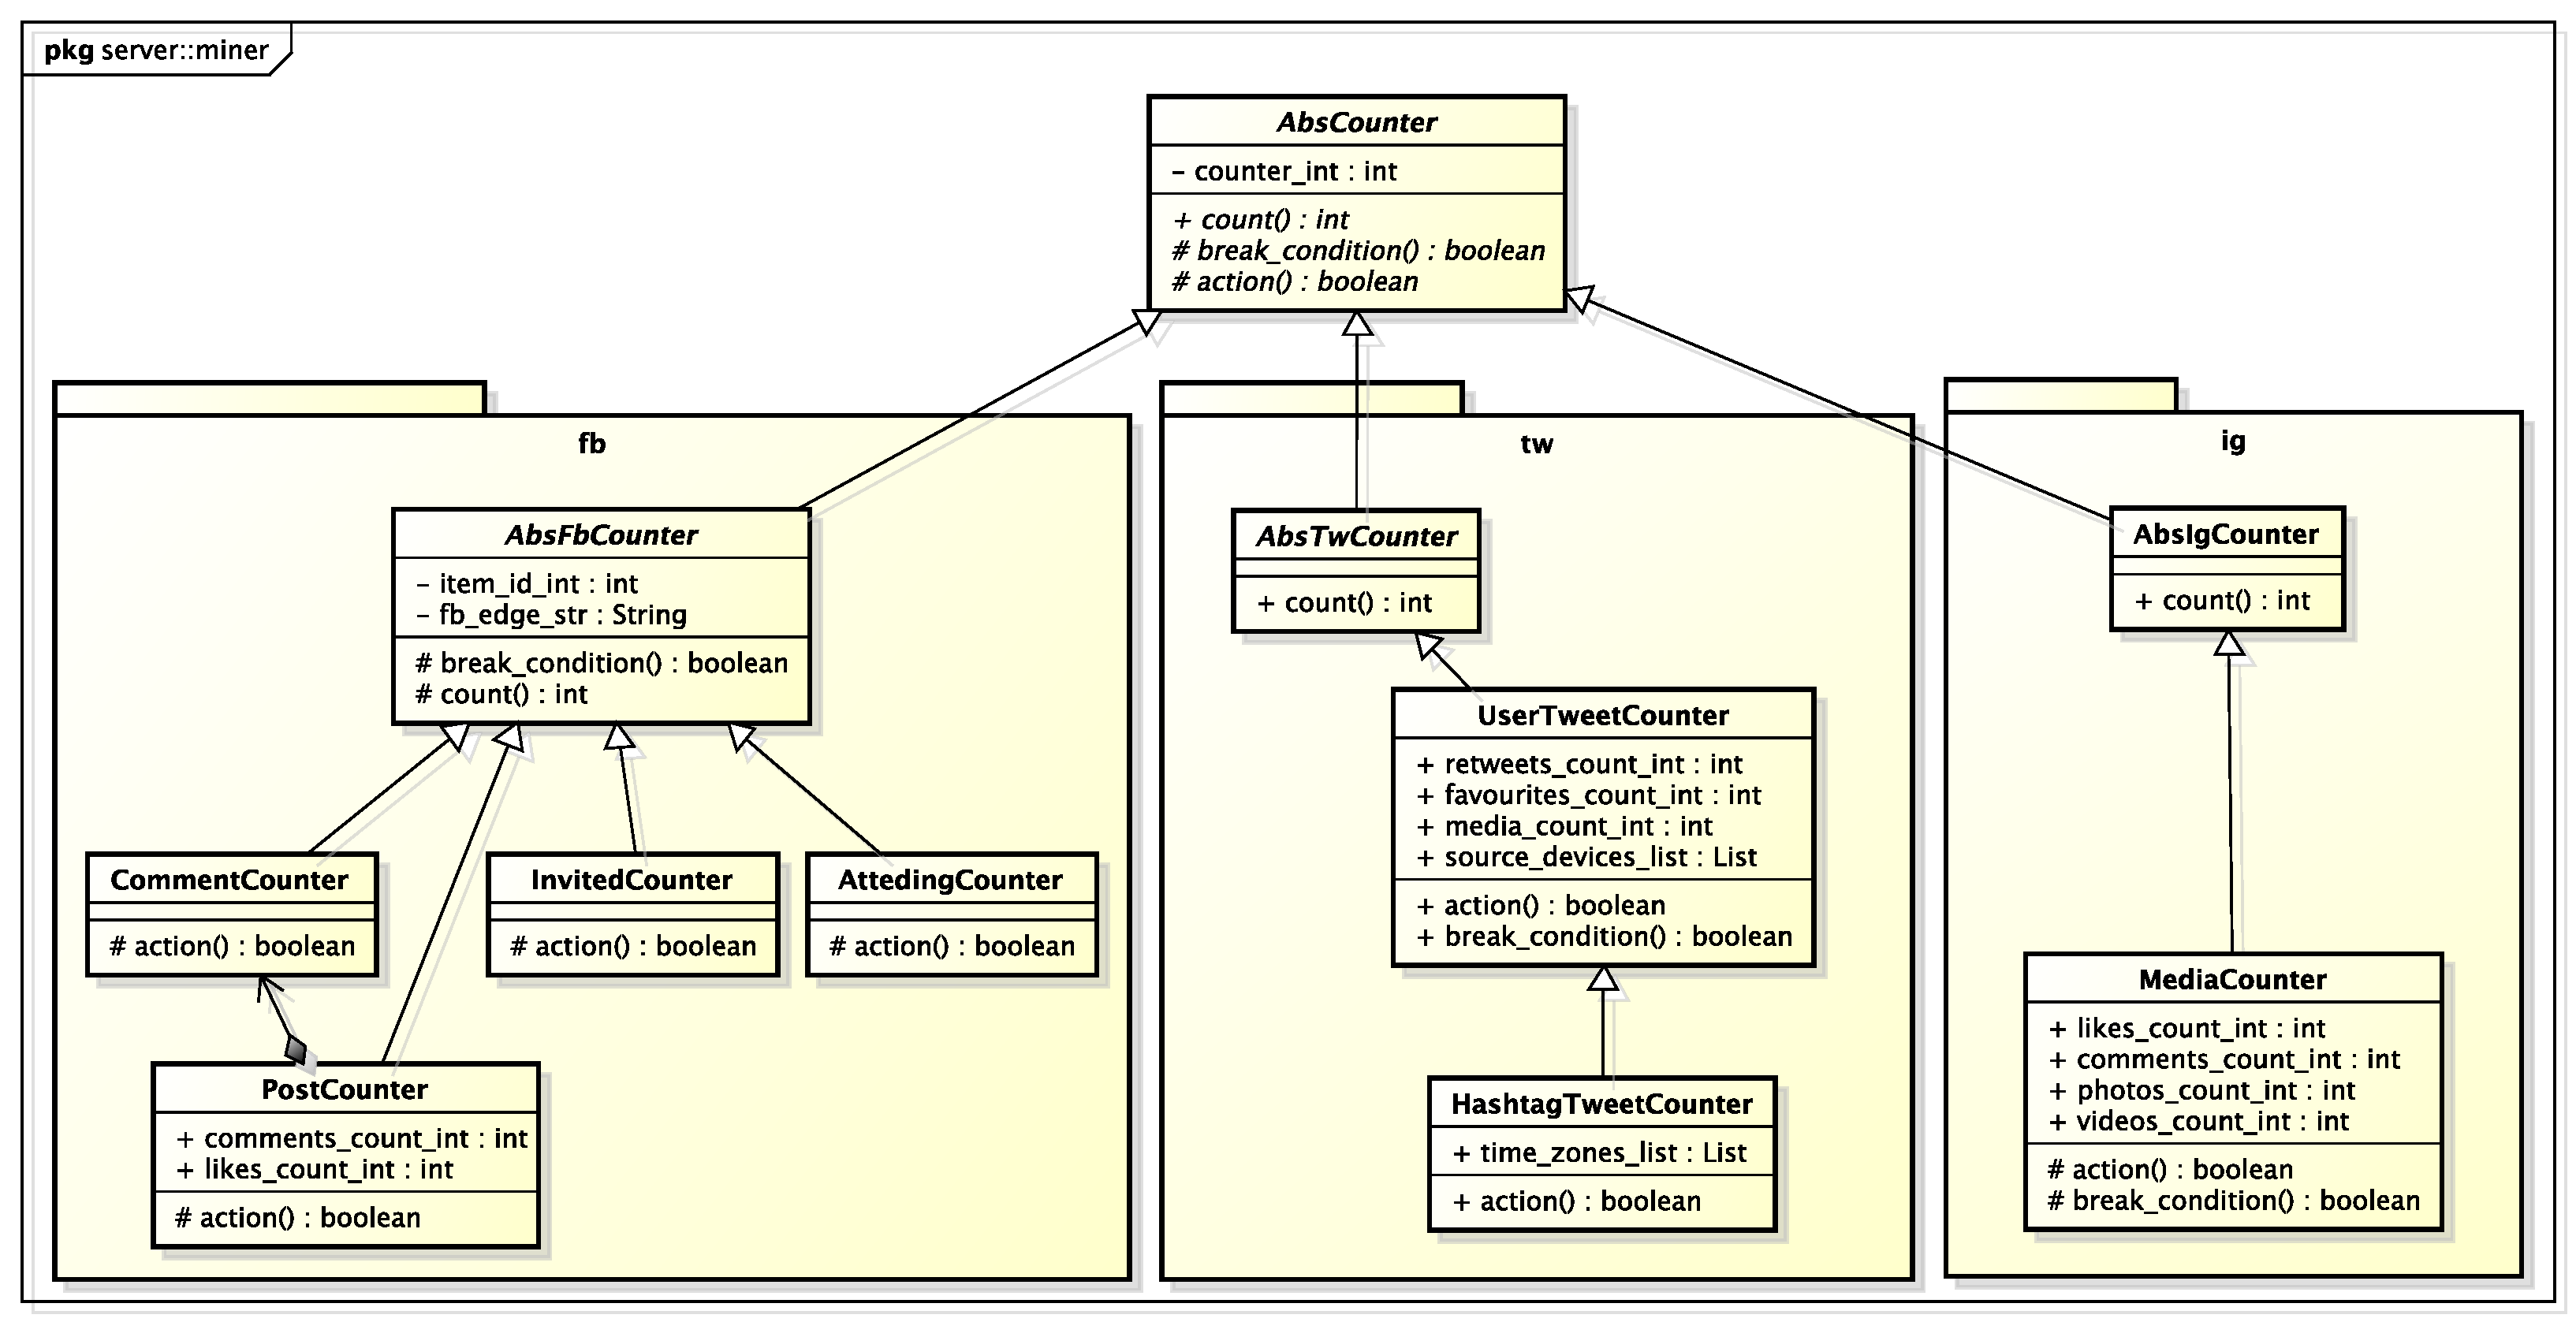
\includegraphics[scale=0.30]{./images/design_pattern_server/dp_template_method.pdf}}
						\caption{Contestualizzazione Template Method - Server}
					\end{figure}
				\end{itemize}
		\end{itemize}
	% subsubsection template_method (end)

% subsection design_pattern_comportamentali (end)
